% !TEX encoding = UTF-8 Unicode

\documentclass[a4paper]{article}

\usepackage{color}
\usepackage{url}
\usepackage[T2A]{fontenc} % enable Cyrillic fonts
\usepackage[utf8]{inputenc} % make weird characters work
\usepackage{graphicx}

\usepackage[english,serbian]{babel}
%\usepackage[english,serbianc]{babel} %ukljuciti babel sa ovim opcijama, umesto gornjim, ukoliko se koristi cirilica

\usepackage[unicode]{hyperref}
\hypersetup{colorlinks,citecolor=green,filecolor=green,linkcolor=blue,urlcolor=blue}

%\newtheorem{primer}{Пример}[section] %ćirilični primer
\newtheorem{primer}{Primer}[section]

\begin{document}

\title{Naslov seminarskog rada\\ \small{Seminarski rad u okviru kursa\\Metodologija stručnog i naučnog rada\\ Matematički fakultet}}

\author{Prvi autor, drugi autor (treći autor)\\ kontakt email prvog, drugog (trećeg) autora}
\date{9.~april 2015.}
\maketitle

\abstract{
U ovom tekstu je ukratko prikazana osnovna forma seminarskog rada. Obratite pažnju da je pored ove .pdf datoteke, u prilogu i odgovarajuća .tex datoteka, kao i .bib datoteka korišćena za generisanje literature. Na prvoj strani seminarskog rada su naslov, apstrakt i sadržaj, i to sve mora da stane na prvu stranu! Kako bi Vaš seminarski zadovoljio standarde i očekivanja, koristite uputstva i materijale sa predavanja na temu pisanja seminarskih radova. Ovo je samo šablon koji se odnosi na fizički izgled seminarskog rada (šablon koji \emph{morate} da ispoštujete!) kao i par tehničkih pomoćnih uputstava. Molim Vas da kada budete predavali seminarski rad, imenujete datoteke tako da sadrže temu seminarskog rada, kao i imena i prezimena članova grupe (ili samo temu i prezimena, ukoliko je sa imenima predugačko). Predaja seminarskih radova biće isključivo preko web forme, a NE slanjem mejla.

\tableofcontents

\newpage

\section{Uvod}
\label{sec:uvod}

Ко жели, може да пише рад ћирилицом. У том случају, неопходно је да су инсталирани одговарајући пакети: texlive-fonts-extra, texlive-latex-extra, texlive-lang-cyrillic, texlive-lang-other. \\

Uz sve novouvedene termine u zagradi naglasiti od koje engleske reči termin potiče. Naredni primeri ilustruju način uvođenja enlegskih termina kao i citiranje.

\begin{primer}
Problem zaustavljanja (eng.~{\em halting problem}) je neodlučiv \cite{haltingproblem}.
\end{primer}

\begin{primer}
Za prevođenje programa napisanih u programskom jeziku C može se koristiti GCC kompajler \cite{gcc}.
\end{primer}

\begin{primer}
 Da bi se ispitivala ispravost softvera, najpre je potrebno precizno definisati njegovo ponašanje \cite{laski2009software}. 
\end{primer}

Reference koje se koriste u ovom tekstu zadate su u datoteci {\em seminarski.bib}. Prevođenje u pdf format u Linux okruženju može se uraditi na sledeći način:
\begin{verbatim}
pdflatex TemaImePrezime.tex 
bibtex TemaImePrezime.aux 
pdflatex TemaImePrezime.tex 
pdflatex TemaImePrezime.tex 
\end{verbatim}
Prvo latexovanje je neophodno da bi se generisao {\em .aux} fajl. {\em bibtex} proizvodi odgovarajući {\em .bbl} fajl koji se koristi za generisanje literature. 
Potrebna su dva prolaza (dva puta pdflatex) da bi se reference ubacile u tekst (tj da ne bi ostali znakovi pitanja umesto referenci). Dodavanjem novih referenci potrebno je ponoviti ceo postupak.  


Broj naslova i podnaslova je proizvoljan. Neophodni su samo Uvod i Zaključak. Na poglavlja unutar teksta referisati se po potrebi. 
\begin{primer}
U odeljku \ref{sec:naslov1} precizirani su osnovni pojmovi, dok su zaključci dati u odeljku \ref{sec:zakljucak}.
\end{primer}

Još jednom da napomenem da nema razloga da pišete:
\begin{verbatim}
\v{s} i \v{c} i \'c ...
\end{verbatim}
Možete koristiti srpska slova
\begin{verbatim}
š i č i ć ... 
\end{verbatim}


Ovde pišem uvodni tekst.
Ovde pišem uvodni tekst. 
Ovde pišem uvodni tekst. 
Ovde pišem uvodni tekst. 


\section{Slike i tabele}
\label{slike_i_tabele}

Slike i tabele treba da budu u svom okruženju, sa odgovarajućim naslovima, obeležene labelom da koje omogućava referenciranje. 

\begin{primer} Ovako se ubacuje slika. Obratiti pažnju da je dodato i 
\begin{verbatim}
\usepackage{graphicx}
\end{verbatim}

\begin{figure}[h!]
\begin{center}
%\includegraphics[scale=0.75]{panda.jpg}
\end{center}
\caption{Pande}
\label{fig:pande}
\end{figure}

Na svaku sliku neophodno je referisati se negde u tekstu. Na primer, na slici \ref{fig:pande} prikazane su pande. 
\end{primer}

\begin{primer} I tabele treba da budu u svom okruženju, i na njih je neophodno referisati se u tekstu. Na primer, u tabeli \ref{tab:tabela1} su prikazana različita poravnanja u tabelama.

\begin{table}[h!]
\begin{center}
\caption{Razlčita poravnanja u okviru iste tabele ne treba koristiti jer su nepregledna.}
\begin{tabular}{|c|l|r|} \hline
centralno poravnanje& levo poravnanje& desno poravnanje\\ \hline
a &b&c\\ \hline
d &e&f\\ \hline
\end{tabular}
\label{tab:tabela1}
\end{center}
\end{table}

\end{primer}





\section{Prvi naslov}
\label{sec:naslov1}


Ovde pišem tekst. 
Ovde pišem tekst. 
Ovde pišem tekst. 
Ovde pišem tekst. 
Ovde pišem tekst. 
Ovde pišem tekst. 
Ovde pišem tekst. 
Ovde pišem tekst. 


\subsection{Prvi podnaslov}
\label{subsec:podnaslov1}

Ovde pišem tekst. 
Ovde pišem tekst. 
Ovde pišem tekst. 
Ovde pišem tekst. 
Ovde pišem tekst. 
Ovde pišem tekst. 
Ovde pišem tekst. 

\subsection{Drugi podnaslov}
\label{subsec:podnaslov2}

Ovde pišem tekst. 
Ovde pišem tekst. 
Ovde pišem tekst. 
Ovde pišem tekst. 
Ovde pišem tekst. 
Ovde pišem tekst. 

\section{Drugi naslov}
\label{sec:naslov2}

Ovde pišem tekst. 
Ovde pišem tekst. 
Ovde pišem tekst. 
Ovde pišem tekst. 

\subsection{... podnaslov}
\label{subsec:podnaslovN}

Ovde pišem tekst. 
Ovde pišem tekst. 
Ovde pišem tekst. 
Ovde pišem tekst. 
Ovde pišem tekst. 
Ovde pišem tekst. 

\section{n-ti naslov}
\label{sec:naslovN}

Ovde pišem tekst. 
Ovde pišem tekst. 
Ovde pišem tekst. 
Ovde pišem tekst. 
Ovde pišem tekst. 

\subsection{... podnaslov}
\label{subsec:podnaslovK}

Ovde pišem tekst. 
Ovde pišem tekst. 
Ovde pišem tekst. 
Ovde pišem tekst. 
Ovde pišem tekst. 

\subsection{... podnaslov}
\label{subsec:podnaslovM}

Ovde pišem tekst. 
Ovde pišem tekst. 
Ovde pišem tekst. 
Ovde pišem tekst. 
Ovde pišem tekst. 

\section{Poslednji naslov}
\label{sec:naslovM}

Ovde pišem tekst. 
Ovde pišem tekst. 
Ovde pišem tekst. 
Ovde pišem tekst. 
Ovde pišem tekst. 
Ovde pišem tekst. 
Ovde pišem tekst. 
Ovde pišem tekst. 
Ovde pišem tekst. 

\section{Sakupljač otpadaka}
\label{sec:djubretar}

%Izvršavanje programa na računaru praćeno je stvaranjem brojnih struktura podataka (objekata).
%Neke od njih generiše sam program, dok su druge vezane za njegovu implementaciju. Sve te strukture podataka se skladište u deo memorije koji se naziva heap.

Strukture podataka koje su alocirane na \textit{hipu} (engl. \textit{heap}), a nisu dostižne preko nekog niza pokazivača programskih promenljivih, nazivaju se \textit{otpaci} (engl. \textit{garbage}). Memorija koju zauzimaju otpaci treba da bude dostupna za alociranje novih struktura podataka. Proces eliminisanja otpadaka, odnosno, njihovog uklanjanja iz memorije naziva se \textbf{sakupljanje otpadaka} (engl. \textit{garbage collection}) i događa se u fazi izvršavanja programa.

\subsection{Motivacija}

Kod proceduralnih programskih jezika, kakav je na primer PASCAL, operacije stvaranja i uništavanja objekata koji se skladište na hipu izvršavaju se eksplicitnim navođenjem određenih naredbi (NEW i DISPOSE) u izvornom k\^odu. To znači da je odgovornost za recikliranje otpadaka na programeru, koji mora da uništi svaki nepotrebni objekat odgovarajućom naredbom i time oslobodi memorijske ćelije zauzete tim objektom. Ukoliko to ne uradi kapacitet memorije se prividno smanjuje. Ova pojava se naziva \textit{curenje memorije} (engl. \textit{memory leak}).

Ovakav koncept je prihvatljiv kod proceduralnih jezika, kod kojih su pomenute operacije retke, ali je neefikasan kada su u pitanju funkcionalni jezici koji se odlikuju čestim izvršavanjem tih operacija \cite{appel}. Zato je kod funkcionalnih programskih jezika posao sakupljanja otpadaka poveren delu sistema za upravljanje memorijom koji se naziva \textit{sakupljač otpadaka} (engl. \textit{garbage collector}).

Različitih tipova sakupljača otpadaka ima mnogo. U daljem tekstu biće predstavljeni neki od njih, kao i njihove osnovne karakteristike.

\subsection{Markirajući sakupljač otpadaka}

Markirajući sakupljač otpadaka je najstariji tip sakupljača otpadaka. Razvijen je početkom 1960-ih godina u okviru programskog jezika LISP \cite{mcca60}.

Programske promenljive i strukture podataka alocirane na hipu formiraju usmeren graf. Promenljive predstavljaju koren tog grafa.

\begin{definicija}
	Kažemo da je čvor \textit{n} \textit{dostižan} u grafu ukoliko postoji put $r\rightarrow \dots \rightarrow n$ od nekog korena \textit{r}.
\end{definicija}

U prvoj fazi, pretragom grafa u širinu se markiraju svi dostižni čvorovi. Ako čvor nije markiran, onda je otpadak i treba da se realocira. Čišćenje hipa se vrši u drugoj fazi počevši od prve adrese i ide do poslednje, pri čemu se traže čvorovi koji nisu markirani. Dobijeni otpaci se povežu u listu koja se naziva \textit{slobodna lista}. Tokom faze čišćenja uklanjaju se markeri svim markiranim čvorovima, da ne bi došlo do problema pri sledećem sakupljanju otpadaka. Nakon što se izvrši sakupljanje otpadaka, prevedeni program nastavlja sa radom.

Kad god program želi da alocira prostor na hipu, on dobija memoriju iz slobodne liste. Kada slobodna lista postane prazna, to je dobar znak da treba opet da se izvrši sakupljanje otpadaka.

\subsection{Sakupljač otpadaka sa brojanjem referenci}
\label{ref:reference counter}

Ideju za ovaj tip sakupljača otpadaka dao je Collins 1960. godine \cite{col60}. On se primenjuje u sistemima kod kojih je hip baziran na listi. Svaka ćelija u hipu sadrži jednu reč koja se naziva \textit{brojač referenci}. Vrednost te reči je broj referenci na ćeliju, tj. broj pokazivača koji na nju pokazuju. Kada se neki podatak smesti u ćeliju i ona postane aktivna, njen brojač referenci dobija vrednost 1. Ako u toku rada program kreira još neki pokazivač na tu ćeliju, njen brojač povećava vrednost za jedan. Ukoliko se uništi neki pokazivač na ćeliju, brojač smanjuje vrednost za jedan. Ako vrednost brojača postane nula, to znači da ne postoji nijedan pokazivač na tu ćeliju, tj. da joj se ne može pristupiti polazeći od nekog korenog pokazivača, pa ona više nije aktivna. Čim ćelija postane neaktivna, reciklira se i to tako što se povezuje u listu slobodnih ćelija.

Ovim se izbegavaju dugotrajni procesi traženja aktivnih ćelija i recikliranja neaktivnih, koji su karakteristični za ostale tipove sakupljača otpadaka. Sve ovo omogućava da se recikliranje otpadaka obavlja paralelno sa izvršavanjem programa, pa je ovaj tip sakupljača pogodan za sisteme u realnom vremenu.

\subsection{Prepisujući sakupljač otpadaka}

Algoritam za ovaj tip sakupljača otpadaka dali su 1969. godine Fenichel i
Yochelson \cite{feni69}. Dostižni deo hipa je usmereni graf, memorijske ćelije su čvorovi, pokazivači su grane, a promenljive su koren.

Prepisujući sakupljač otpadaka prolazi kroz deo grafa koji je alociran na hipu, praveći izomorfnu kopiju u svežem delu hipa. Taj sveži deo je kompaktan i podaci zauzimaju kontinualan blok memorije, bez fragmentacije. Koren sada pokazuje na kopiju, a original se oslobađa. 

Slika \ref{fig:copygc} prikazuje situaciju pre i posle prepisujućeg sakupljanja. Pre sakupljanja, početni prostor je bio pun dostižnih čvorova i otpadaka, nije ostalo mesta za alociranje jer je dostignut limit. Nakon sakupljanja novi prostor između alociranih čvorova i limita je slobodan za alociranje.

\begin{figure}[h]
	\centering
	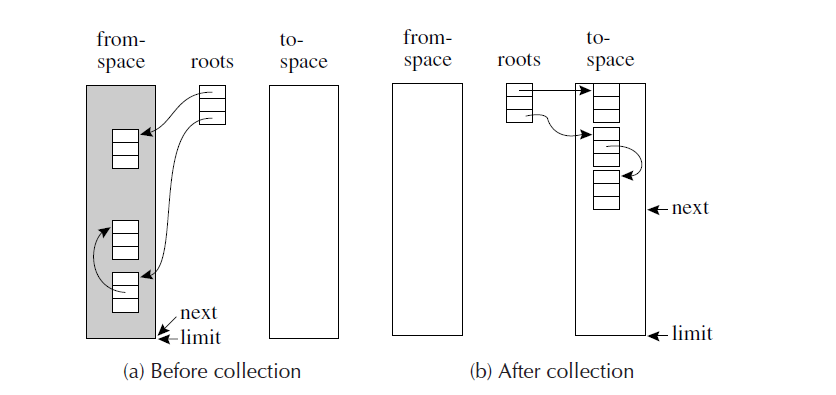
\includegraphics[width=0.9\textwidth]{copygc.png}
	\caption{Prepisujući sakupljač otpadaka.}
	\label{fig:copygc}
\end{figure}

\subsection{Generacijski sakupljač otpadaka}

Jedna od mana prepisujućeg sakupljača otpadaka je što u svakom ciklusu sakupljanja otpadaka premešta sve aktivne ćelije izvornog dela, odnosno, objekte smeštene u njima. To znači da će objekti koji imaju duži životni vek biti premeštani više puta, u toku više ciklusa sažimanja. Ovo ponovljeno premeštanje predstavlja nepotreban posao, koji se može izbeći tako što će se hip podeliti na dva dela.

U jednom delu hipa će se smeštati objekti dužeg životnog veka, što znači da će u njemu biti manje otpadaka, te će proces njihovog sakupljanja moći ređe da se vrši. Drugi će sadržati objekte kraćeg životnog veka i zbog toga će imati veći broj otpadaka, pa će se kompakcija vršiti češće. Strategija koja određuje koliko će se često neki region sažimati naziva se \textit{politika sakupljanja} (engl. \textit{collection policy}).

Postavlja se pitanje kako odrediti koji objekti imaju duži životni vek, tj. kako odrediti koji će se objekti smeštati u koji deo hipa. Empirijske metode su pokazale da većina mladih objekata (onih koji su skoro kreirani) predstavlja privremene strukture ili međurezultate i da samim tim ti objekti imaju kratak životni vek \cite{app87}. Samo mali broj objekata je deo neke strukture dugog životnog veka.

U mnogim stilovima programiranja, kada se kreira objekat A, njegova polja se odmah inicijalizuju i recimo da A pokazuje na objekte B i C. Da bi to bilo moguće objekti B i C moraju već postojati, tako da imamo noviji objekat koji pokazuje na starije objekte. Jedini način da stariji objekat B pokazuje na noviji objekat A je ukoliko je neko polje objekta B izmenjeno dugo nakon kreiranja samog objekta, što je empirijski veoma retko.

\iffalse
\subsection{Odnos prema kompilatoru}

Kompilator za jezik sa sakupljanjem otpadaka uzajamno dejstvuje sa sakupljačem otpadaka generišući k\^od za alociranje podataka, opisujući lokacije za koren svakog ciklusa sakupljanja otpadaka i opisujući izgled podataka na hipu (da li je lista, stek ili stablo). Neki programski jezici i programi, veoma brzo alociraju memoriju na hipu (i generišu otpatke). Ovo je posebno istaknuto kod funkcionalnih programskih jezika, gde je obeshrabreno menjanje starijih podataka.
\fi

% TODO: pročitajte i dajte svoj sud
% ovo poglavlje je nezvanicno završeno
% potencijalno treba da se dopuni ili lepše zapiše da bi sve delovalo kao jedna celina

\section{Polimorfna provera tipova}
\label{sec:provera tipova}


%The Implementation of Functional Programming Languages strana 139
Neki moderni jezici, kao što je Miranda, imaju svojstvo koje omogućava programeru da ne navodi tipove objekata koje definiše u programu. Kompilator može da odredi tipove ako je to moguće. Deo kompilatora koji se bavi ovim poslom naziva se \textit{zaključivač tipova} \cite{the-implementation-of-functional-programming-languages}. Proveravač tipova je od velike koristi programeru jer mu ukazuje na greške, od trivijalnih propusta u kucanju do velikih logičkih grešaka. Pomaže u pisanju robusnih programa kao i u izgradnji bržih implementacija programskih jezika. Ako zaključivač tipova obradi program, pri izvršavanju se neće javiti greške poput upotrebe promenljive tipa bool kao da je tipa int.
\\
\\ %BasicTypechecking.pdf str. 6
% potrebna referenca za unifikaciju

Izrazi koji sadrže nekoliko pojavljivanja istog tipa, kao $\alpha \longrightarrow \alpha$, izražavaju kontekstnu zavisnost, u ovom slučaju to je zavisnost domena i kodomena tipa funkcije. Proces zaključivanja tipova sastoji se od uparivanja tipova operatora i instanciranja tipova promenljivih. Kad god se tip promenljive instancira, sve ostale pojave iste promenljive moraju biti instancirane sa istom vrednošću: ispravna instanciranja izraza $\alpha \longrightarrow \alpha$ su $int \longrightarrow int$,  $bool \longrightarrow bool$, itd. Proces kontekstnog instanciranja izvodi se pomoću \textit{unifikacije} i ona je osnova polimorfne provere tipova. Unifikacija ne uspeva kada pokušava da upari dva operatora različitih tipova (npr. int i bool) ili kada pokušava da instancira promenljivu izrazom koji sadrži tu promenljivu (npr. $a$ i $a\longrightarrow b$, gde će se napraviti rekurzija bez izlaza) \cite{basic-typechecking}. %The latter situation arises in typechecking self-application (e.g. fun(x) x(x)), which is therefore considered illegal.
U opštem slučaju, tip izraza određuje se pomoću skupa pravila kombinovanja tipova za jezičke konstrukcije i tipova primitivnih operatora. 

\iffalse
%The Implementation of Functional Programming Languages sekcija 8.1
\subsection{Ukratko o notaciji}
%ovo je sve nebitno zapravo, ali neka stoji za sad :D
Tipovi koji su zanimljivi kada je funkcionalno programiranju u pitanju su karakteri, broj, istinitosna vrednost, kao i tipovi torki, lista i funkcija. Kada govorimo o ovim tipovima, koristićemo sledeću notaciju:
$$a::A$$

\noindent što predstavlja promenljivu $a$ koja je tipa $A$. 	
\\
\\ Ako su dati tipovi $A_1, \ldots, A_n$ onda $(A_1, \ldots, A_n)$ predstavlja tip tokre $(a_1, \ldots, a_n)$ za koji važi $a_1::A_1$ i $a_n::A_n$. Bitno je naglasiti da $A_1, \ldots, A_n$ ne predstavljaju iste tipove, odnosno da koordinate jedne torke ne moraju biti sve istog tipa. Takođe, tip torke određuje broj koordinata (odnosno dimenziju torke) i njihove tipove. 
\\
\\ Ako je dat tip $A$ onda je $[B]$ tip liste čiji su elementi tipa $B$. U slučaju da su elementi liste torke, sve torke moraju biti istog tipa. Za razliku od tipa torke, tip liste ne određuje njenu dužinu. 
\\
\\ Ako su dati tipovi $A$ i $B$ koristimo $A \longrightarrow B$ za zapis tipa funkcije $f$ koja se primenjuje na promenljivu $a::A$, a čije vrednosti $(f \quad a)$ su tipa $B$.


\fi 


%BasicTypechecking.pdf str. 9
\subsection{Zaključivanje tipova}
\label{subsec: zakljucivanje tipova}

Osnovni algoritam za zaključivanje tipova opisan je u nastavku \cite{basic-typechecking}.

\begin{enumerate}
	\item Kada se pojavi nova promenljiva $x$, njoj se dodeljuje novi tip promenljive što znači da joj tip mora biti određen u daljem kontekstu u kom se pojavljuje. Par $<x, a>$ se čuva u okruženju koje se pretražuje svaki put kad se pojavi $x$, u kom je $x$ tipa $a$.
	
	\item Kad imamo uslovno grananje, izraz u \textit{if} se uparuje sa bool, dok se \textit{then} i \textit{else} grane ostavljaju nedefinisane kako bi se odredio jedinstven tip za ceo izraz.
	
	\item U apstrakciji $\lambda x.e$, tip za $e$ se zaključuje u kontekstu gde je $x$ povezan sa novim tipom promenljive.
	
	\item U aplikaciji $f(a)$, tip od f se unifikuje sa tipom $A \longrightarrow b$, gde je $A$ tip parametra $a$, dok je $b$ nova tipska promenljiva. Ovo ukazuje na to da $f$ mora biti tipa funkcije čiji domen se unifikuje sa $A$, a $b$ je tip povratne vrednosti.
\end{enumerate}





\section{Zaključak}
\label{sec:zakljucak}

Ovde pišem zaključak. 
Ovde pišem zaključak. 
Ovde pišem zaključak. 
Ovde pišem zaključak. 
Ovde pišem zaključak. 
Ovde pišem zaključak. 
Ovde pišem zaključak. 
Ovde pišem zaključak. 
Ovde pišem zaključak. 
Ovde pišem zaključak. 
Ovde pišem zaključak. 
Ovde pišem zaključak. 



\addcontentsline{toc}{section}{Literatura}
\appendix
\bibliography{seminarski} 
\bibliographystyle{plain}

\appendix
\section{Dodatak}
Ovde pišem dodatne stvari, ukoliko za time ima potrebe.
Ovde pišem dodatne stvari, ukoliko za time ima potrebe.
Ovde pišem dodatne stvari, ukoliko za time ima potrebe.
Ovde pišem dodatne stvari, ukoliko za time ima potrebe.
Ovde pišem dodatne stvari, ukoliko za time ima potrebe.



\end{document}
